\documentclass[aspectratio=169]{beamer}
\usetheme{Madrid}

\setbeamertemplate{navigation symbols}{}

\usefonttheme[onlymath]{serif}

\AtBeginSection[]{
  \begin{frame}
  \vfill
  \centering
  \begin{beamercolorbox}[sep=8pt,center,shadow=true,rounded=true]{title}
    \usebeamerfont{title}\insertsectionhead\par%
  \end{beamercolorbox}
  \vfill
  \end{frame}
}

\usepackage{bm}
\usepackage{xifthen}

\DeclareMathOperator*{\KLOp}{KL}
\DeclareMathOperator*{\PrOp}{\mathbb{P}}
\DeclareMathOperator*{\EvOp}{\mathbb{E}}
\DeclareMathOperator*{\VarOp}{\mathbb{V}ar}

\newcommand{\CD}{\mathcal{D}}
\newcommand{\CH}{\mathcal{H}}
\newcommand{\CX}{\mathcal{X}}
\newcommand{\CY}{\mathcal{Y}}

\newcommand{\RR}{\mathbb{R}}

\newcommand*{\KL}[2]{\KLOp(#1\parallel#2)}

\renewcommand*{\Pr}[2][]{%
  \mathchoice{%
    \PrOp\ifthenelse{\isempty{#1}}{}{_{#1}}\left[#2\right]%
  }{%
    \PrOp\ifthenelse{\isempty{#1}}{}{_{#1}}[#2]%
  }{%
    \PrOp\ifthenelse{\isempty{#1}}{}{_{#1}}[#2]%
  }{%
    \PrOp\ifthenelse{\isempty{#1}}{}{_{#1}}[#2]%
  }%
}
\newcommand*{\Ev}[2][]{%
  \mathchoice{%
    \EvOp\ifthenelse{\isempty{#1}}{}{_{#1}}\left[#2\right]%
  }{%
    \EvOp\ifthenelse{\isempty{#1}}{}{_{#1}}[#2]%
  }{%
    \EvOp\ifthenelse{\isempty{#1}}{}{_{#1}}[#2]%
  }{%
    \EvOp\ifthenelse{\isempty{#1}}{}{_{#1}}[#2]%
  }%
}
\newcommand*{\Var}[2][]{%
  \mathchoice{%
    \VarOp\ifthenelse{\isempty{#1}}{}{_{#1}}\left[#2\right]%
  }{%
    \VarOp\ifthenelse{\isempty{#1}}{}{_{#1}}[#2]%
  }{%
    \VarOp\ifthenelse{\isempty{#1}}{}{_{#1}}[#2]%
  }{%
    \VarOp\ifthenelse{\isempty{#1}}{}{_{#1}}[#2]%
  }%
}

\title{PAC-Bayes Theory and Bayesian Inference}
\author{Saibal De}
\date{April 19, 2020}

\begin{document}

\begin{frame}
  \titlepage
\end{frame}

\begin{frame}{Outline}
  \begin{enumerate}
    \item
      Introduction
    \item
      Bayesian Inference
    \item
      PAC-Bayes Theory
    \item
      PAC Bayesian Inference
    \item
      Conclusion
  \end{enumerate}
\end{frame}

\section{Introduction}

\begin{frame}{Motivation}
  \begin{itemize}
  	\item
      PAC theory offers uniform guarantees on learnability
      \begin{itemize}
        \item
          Applicable primarily to classification problems
        \item
          Needs finite VC dimension hypothesis classes
      \end{itemize}
  	\item
      Bayesian inference provides unified framework for data-driven learning
      \begin{itemize}
        \item
          Works very well in practice
        \item
          Does not provide uniform guarantees on generalization error
      \end{itemize}
  	\item
      How do we unify these two learning frameworks?
  \end{itemize}
\end{frame}

\begin{frame}{Summary of Main Results}
	\begin{itemize}
		\item
      We develop uniform empirical learning guarantees for Bayesian inference
      tasks
    \item
      We apply this theory to Bayesian linear regression
	\end{itemize}
\end{frame}

\section{Bayesian Inference}

\begin{frame}{Main Mechanism}
  \begin{itemize}
    \item
      Goal: Estimate model parameter $\theta$ from data $S$ generated from model
    \item
      Assume prior distribution $p(\theta)$ on parameter space
    \item
      Compute likelihood $p(S \mid \theta)$ from the model
    \item
      Use Bayes rule to compute posterior
      \begin{equation*}
        p(\theta \mid S) = \frac{p(\theta) p(S \mid \theta)}{p(S)}
      \end{equation*}
    \item
      We simply need to construct the posterior:
      \begin{itemize}
        \item
          Analytic methods: Conjugate priors
        \item
          Sampling methods: Markov Chain Monte-Carlo (MCMC)
        \item
          Approximate methods: Variational Bayes (VB)
      \end{itemize}
  \end{itemize}
\end{frame}

\begin{frame}{Bayesian Linear Regression}
  \begin{itemize}
    \item
      Goal: Given points $S = \{(x_i, y_i) : 1 \leq i \leq n\}$, find function
      $f : [0, 1] \to \RR$ to fit data
    \item
      Model
      \begin{equation*}
        h_{\bm{\theta}}(x) = \sum_{i = 1}^m \theta_i \phi_i(x) + \eta =:
        \bm{\phi}(x)^\top \bm{\theta} + \eta, \quad \eta \sim \mathcal{N}(0,
        \sigma_\eta^2)
      \end{equation*}
    \item
      Bayesian inference:
      \begin{itemize}
        \item
          Prior $p(\bm{\theta}) = \mathcal{N}(\bm{\theta} \mid \bm{0},
          \sigma_\theta^2
          \mathbf{I}_m)$
        \item
          Likelihood $p(S \mid \bm{\theta}) = p(\bm{x}) p(\bm{y} \mid \bm{x},
          \bm{\theta}) = p(\bm{x}) \mathcal{N}(\bm{y} \mid
          \mathbf{\Phi}(\bm{x})^\top \bm{\theta}, \sigma_\eta^2 \mathbf{I}_n)$
        \item
          Posterior $p(\bm{\theta} \mid S) = \mathcal{N}(\bm{\theta} \mid
          \bm{\mu}, \mathbf{\Sigma})$
      \end{itemize}
      Here
      \begin{equation*}
        \mathbf{\Phi}(\bm{x}) =
        \begin{bmatrix}
          \bm{\phi}(x_1) & \cdots & \bm{\phi}(x_n)
        \end{bmatrix},
        \quad \mathbf{\Sigma}^{-1} = \frac{1}{\sigma_\theta^2} \mathbf{I}_m +
        \frac{1}{\sigma_\eta^2} \mathbf{\Phi}(\bm{x})
        \mathbf{\Phi}(\bm{x})^\top,
        \quad \bm{\mu} = \frac{1}{\sigma_\eta^2} \mathbf{\Sigma}
        \mathbf{\Phi}(\bm{x}) \bm{y}
      \end{equation*}
  \end{itemize}
\end{frame}

\begin{frame}{Bayesian Linear Regression}
  \centering
  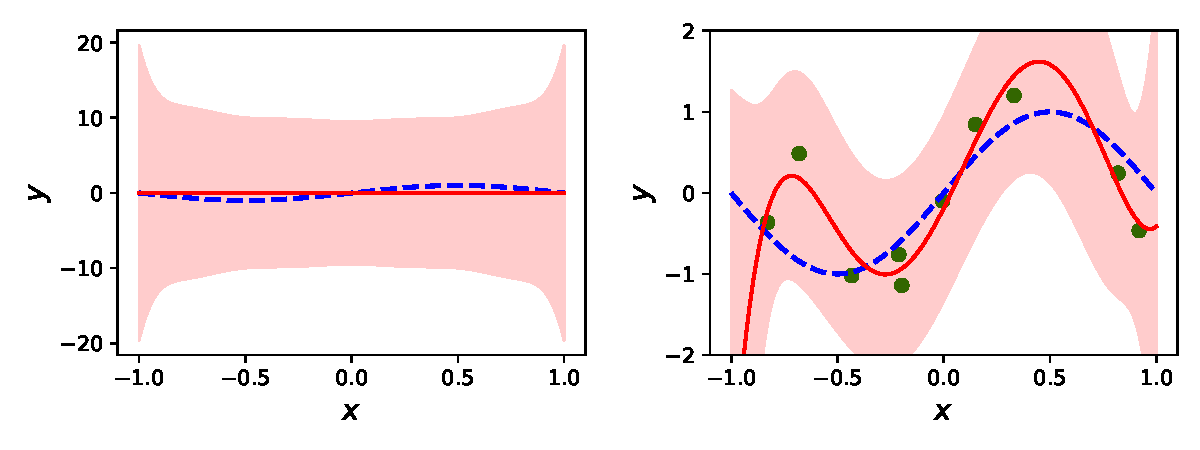
\includegraphics[width=\textwidth]{../figures/bayesian_regression_1.pdf}

  Bayesian inference with 10 samples
\end{frame}

\begin{frame}{Bayesian Linear Regression}
  \centering
  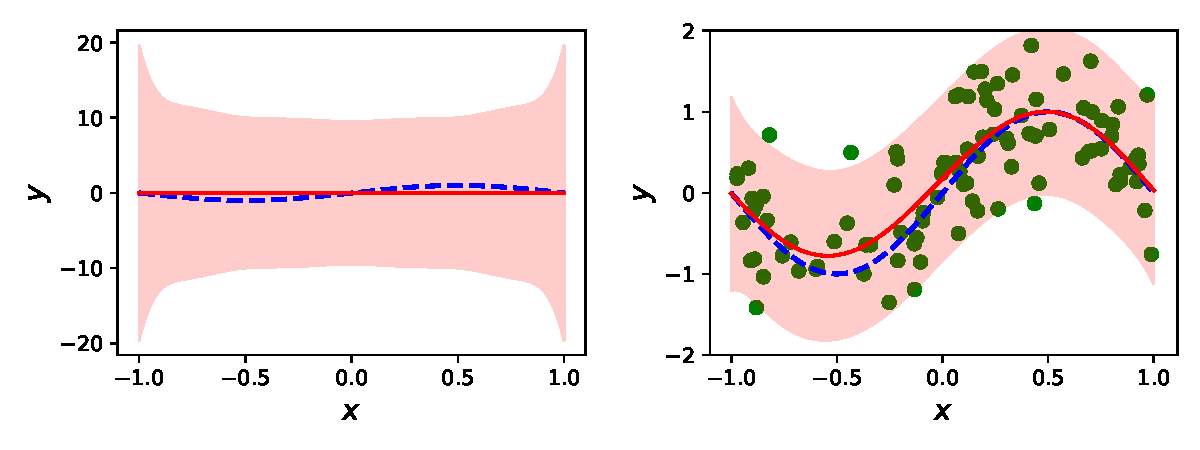
\includegraphics[width=\textwidth]{../figures/bayesian_regression_3.pdf}

  Bayesian inference with 100 samples
\end{frame}

\section{PAC-Bayes Theory}

\begin{frame}{Statistical Learning Setup}
  \begin{itemize}
    \item
      Feature space $\CX$
    \item
      Label space $\CY$
    \item
      Sample $S = \{(x_1, y_1), \ldots, (x_n, y_n)\}$ drawn i.i.d.\ from
      distribution $\CD$ on $\CX \times \CY$
    \item
      Hypothesis set $\CH$ of functions of the form $h : \CX \to \CY$
    \item
      Loss function $L : \CH \times \CX \times \CY \to \RR$
    \item
      Training error $\hat{R}_S^L(h) = \frac{1}{n} \sum_{i = 1}^n L(h, x_i,
      y_i)$
    \item
      Generalization error $R_\CD^L(h) = \Ev[(x, y) \sim \CD]{L(h, x, y)}$
  \end{itemize}
\end{frame}

\begin{frame}{General PAC-Bayes Approach}
  \begin{itemize}
    \item
      Main Mechanism
      \begin{itemize}
        \item
          Impose prior distribution $\pi$ on $\CH$
        \item
          Observe data $S$
        \item
          Learning algorithm returns posterior distribution $\hat{\rho}$ on $\CH$
      \end{itemize}
    \item
      Need to balance
      \begin{itemize}
        \item
          Average training error $\Ev[h \sim \hat{\rho}]{\hat{R}_S^L(h)}$
        \item
          Average generalization error $\Ev[h \sim \hat{\rho}]{R_\CD^L(h)}$
      \end{itemize}
  \end{itemize}
\end{frame}

\begin{frame}{A General Form of PAC-Bayes Bounds}
  \begin{theorem}[General PAC-Bayes Bound]
    $\CX$, $\CY$, $S$, $\CH$, $\pi$, loss function $L : \CH \times \CX \times
    \CY \to I$ with interval $I \subseteq \RR$, convex function $\Delta : I
    \times I \to \RR$, real number $\delta \in (0, 1)$. Then following holds
    with probability at least $1 - \delta$ over $S \sim \CD^n$
    \begin{equation*}
      \Delta\left(\Ev[h \sim \rho]{R_\CD^L(h)}, \Ev[h \sim
      \rho]{\hat{R}_S^L(h)}\right) \leq \frac{1}{n} \left[\KL{\rho}{\pi} +
      \ln\frac{1}{\delta} + \psi_\Delta^L(\pi, \CD, n)\right]
    \end{equation*}
    where
    \begin{equation*}
      \psi_\Delta^L(\pi, \CD, n) = \ln\left(\Ev[h \sim \pi]{\Ev[S' \sim
      \CD^n]{\exp(n \Delta(R_\CD^L(h), \hat{R}_{S'}^L(h)))}}\right)
    \end{equation*}
    for any distribution $\rho$ on $\CH$
  \end{theorem}
\end{frame}

\begin{frame}{Catoni's PAC-Bayes Bound}
  \begin{theorem}[Catoni's PAC-Bayes Bound]
    $\CX$, $\CY$, $S$, $\CH$, $\pi$, loss function $L : \CH \times \CX \times
    \CY \to [a, b]$, real number $\delta \in (0, 1)$.  Then following holds with
    probability at least $1 - \delta$ over $S \sim \CD^n$
    {
      \small
      \begin{equation*}
        \Ev[h \sim \rho]{R_\CD^L(h)} \leq a + \frac{b - a}{1 - e^{a - b}}\left[1
        - e^{a {\color{red} + a - b}} \exp\left(- \Ev[h \sim
        \rho]{\hat{R}_S^L(h)} - \frac{1}{n} \left[\KL{\rho}{\pi} +
        \ln\frac{1}{\delta}\right]\right)\right]
      \end{equation*}
    }
    for any distribution $\rho$ on $\CH$
  \end{theorem}
  
  Proof: Use
  \begin{equation*}
    \Delta_\beta(s, t) = - \ln \left[1 - (1 - e^{-\beta}) \frac{s - a}{b -
    a}\right] - \beta \frac{t - a}{b - a}, \quad a \leq s, t \leq b, \quad \beta
    > 0
  \end{equation*}
  in the general PAC-Bayes bound and show $\psi_{\Delta_\beta}^L(\pi, \CD, n)
  \leq n \beta$. Substitute $\beta = b - a$.
\end{frame}

\begin{frame}{Optimal Gibbs Posterior}
  \begin{itemize}
    \item
      Fixed $\CX$, $\CY$, $S$, $\CH$, $L$, $\pi$, $\delta$
    \item
      Optimizing the bound implies minimizing
      \begin{equation*}
        \begin{split}
          n \Ev[h \sim \rho]{\hat{R}_S^L(h)} + \KL{\rho}{\pi}
          &= \Ev[h \sim \rho]{n \hat{R}_S^L(h) + \ln\frac{\rho(h)}{\pi(h)}} \\
          &= \Ev[h \sim \rho]{\ln\frac{\rho(h)}{\rho^*(h)}} - \ln Z_S \\
          &= \KL{\rho}{\rho^*} - \ln Z_S
        \end{split}
      \end{equation*}
      where $\rho^*(h) = \frac{1}{Z_S} \pi(h) \exp(-n \hat{R}_S^L(h))$
    \item
      Optimal distribution is $\rho = \rho^*$
  \end{itemize}
\end{frame}

\section{PAC Bayesian Inference}

\begin{frame}{Correspondence between PAC-Bayes and Bayesian Inference}
  \begin{itemize}
    \item
      Parametrize $\CH = \{h_\theta : \theta \in \Theta\}$
    \item
      Loss function $L_\text{nll}(\theta, x, y) = -\log p(x, y \mid \theta)$
    \item
      Data $S$ of i.i.d.\ observations
      \begin{equation*}
        \log p(S \mid \theta) = \sum_{i = 1}^n \log p(x_i, y_i \mid \theta) =
        -\sum_{i = 1}^n L_\text{nll}(\theta, x_i, y_i) = -n
        \hat{R}_S^{L_\text{nll}}(\theta)
      \end{equation*}
    \item
      Posterior
      \begin{equation*}
        p(\theta \mid S) = \frac{\pi(\theta) p(S \mid \theta)}{p(S)} \propto
        \pi(\theta) \exp(-n \hat{R}_S^{L_\text{nll}}(\theta))
      \end{equation*}
      is exactly the optimal Gibbs posterior, provided $L_\text{nll}$ is
      bounded
  \end{itemize}
\end{frame}

\begin{frame}{PAC-Bayes for Unbounded Loss Functions}
  \begin{theorem}[Alquier et al PAC-Bayes Bound]
    $\CX$, $\CY$, $S$, $\CH$, $\pi$, any loss function $L$, real numbers
    $\lambda > 0$ and $\delta \in (0, 1)$. Then following holds with probability
    at least $1 - \delta$ over $S \sim \CD^n$
    \begin{equation*}
      \Ev[h \sim \rho]{R_\CD^L(h)} \leq \Ev[h \sim \rho]{\hat{R}_S^L(h)} +
      \frac{1}{\lambda} \left[\KL{\rho}{\pi} + \ln\frac{1}{\delta} +
      \psi_\lambda^L(\pi, \CD, n)\right]
    \end{equation*}
    where
    \begin{equation*}
      \psi_\lambda^L(\pi, \CD, n) = \ln\left(\Ev[h \sim \pi]{\Ev[S' \sim
      \CD^n]{\exp(\lambda [R_\CD^L(h) - \hat{R}_{S'}^L(h)])}}\right)
    \end{equation*}
    for any distribution $\rho$ on $\CH$
  \end{theorem}

  Proof: General PAC-Bayes theorem with $\Delta(s, t) = \frac{\lambda}{n} (s -
  t)$ and $I = \RR$
\end{frame}

\begin{frame}{Sub-Gamma Loss}
  \begin{definition}[Sub-Gamma Loss]
    A loss function $L : \CH \times \CX \times \CY \to \RR$ is sub-gamma with
    variance factor $s^2$ and scale factor $c$ if w.r.t.\ prior $\pi$ on $\CH$
    and data distribution $\CD$ on $\CX \times \CY$ if
    \begin{equation*}
      \log \Ev[h \sim \pi, (x, y) \sim \CD]{e^{t L(h, x, y)}} \leq
      \frac{s^2}{c^2}(-\ln(1 - t c) - t c) \leq \frac{t^2 s^2}{2 (1 - c t)},
      \quad t \in \left(0, \frac{1}{c}\right)
    \end{equation*}
  \end{definition}
  \begin{corollary}
    $\CX$, $\CY$, $S$, $\CH$, $\pi$, sub-gamma $L$ with variance factor $s^2$
    and scale $c < 1$ and $\delta \in (0, 1)$:
    \begin{equation*}
      \Ev[h \sim \rho]{R_\CD^L(h)} \leq \Ev[h \sim \rho]{\hat{R}_S^L(h)} +
      \frac{1}{n} \left[\KL{\rho}{\pi} + \ln\frac{1}{\delta}\right] + \frac{1}{2
      (1 - c)} s^2
    \end{equation*}
    with probability at least $1 - \delta$ over $S \sim \CD^n$ for any
    distribution $\rho$ on $\CH$
  \end{corollary}
\end{frame}

\begin{frame}{Bayesian Linear Regression, Revisited}
  \begin{itemize}
    \item
      Squared loss function $L(h_{\bm{\theta}}, x, y) = (h_{\bm{\theta}}(x) -
      y)^2$
    \item
      Hypothesis class elements $h_{\bm{\theta}}(x) = \bm{\phi}(x)^\top
      \bm{\theta}$ for $\bm{\theta} \in \RR^m$
    \item
      $\pi(\bm{\theta}) = \mathcal{N}(\bm{0}, \sigma_\theta^2
      \mathbf{I}_m)$
    \item
      $\CD(x, y) = \CD_x(x) \CD_{y \mid x}(y \mid x)$ with
      $\CD_{y \mid x}(y \mid x) = \mathcal{N}(h_{\bm{\theta}^*}(x),
      \sigma_\eta^2)$
    \item
      Loss function sub-gamma$(s, c)$ w.r.t.\ $\pi(\bm{\theta})$ and $\CD(x, y)$
      when
      \begin{equation*}
        c = 2 \kappa_{\bm{\phi},x}^2 \sigma_\theta^2, \quad s^2 = 2
        [\kappa_{\bm{\phi},x}^2 (\sigma_\theta^2 m + \| \bm{\theta}^* \|^2) +
        \sigma_\eta^2 (1 - c)] 
      \end{equation*}
      where
      \begin{equation*}
        \kappa_{\bm{\phi},x}^2 = \left\| \Ev[x \sim \CD_x]{\bm{\phi}(x)
        \bm{\phi}(x)^\top} \right\|_2
      \end{equation*}
  \end{itemize}
\end{frame}

\begin{frame}{Bayesian Linear Regression, Revisited}
  \begin{itemize}
    \item
      Using Legendre polynomials and uniform prior on $x$, we can compute
      $\kappa_{\bm{\phi},x}^2 \leq C \log m$ Then
      \begin{equation*}
        c \leq 2 C \sigma_\theta^2 \log m, \quad s^2 \leq 2 [C (\sigma_\theta^2
        m + \| \bm{\theta}^* \|^2) \log m + \sigma_\eta^2 (1 - c)]
      \end{equation*}
    \item
      The constant term in the bound is $\frac{1}{2(1 - c)} s^2$ and we have the
      constraint $c < 1$
    \item
      As complexity of hypothesis class $m$ increases, we need narrow priors
    \item
      The bound degrades as
      \begin{itemize}
        \item
          Noise variance $\sigma_\eta$ increases
        \item
          Complexity of hypothesis class $m$ increases
        \item
          True parameter $\bm{\theta}^*$ moves away from origin
      \end{itemize}
  \end{itemize}
\end{frame}

\section{Conclusion}

\begin{frame}{Summary}
	\begin{itemize}
		\item
      Described general bounds for PAC-Bayes learning
    \item
      Applied PAC-Bayes theory to Bayesian linear regression
	\end{itemize}
\end{frame}

\begin{frame}{Next Steps}
  \begin{itemize}
    \item
      Different types of loss functions
    \item
      Learning algorithms from the bounds
    \item
      Choice of priors
      \begin{itemize}
        \item
          New developments on data-dependent priors
      \end{itemize}
  \end{itemize}
\end{frame}

\section{References}

\begin{frame}[allowframebreaks]
  \frametitle{References}
  \nocite{*}
  \bibliography{references}
  \bibliographystyle{amsalpha}
\end{frame}

\section{Backup Slides}

\begin{frame}{Bayesian Linear Regression: Posterior Computation}
  \begin{itemize}
    \item
      We compute the posterior
      \begin{equation*}
        \begin{split}
          -\log p(\bm{\theta} \mid S)
          &= -\log p(\bm{\theta}) - \log p(S \mid \bm{\theta}) + \text{const.}
          \\
          &= \frac{1}{2 \sigma_\theta^2} \| \bm{\theta} \|^2 + \frac{1}{2
          \sigma_\eta^2} \| \bm{y} - \mathbf{\Phi}(\bm{x})^\top \bm{\theta} \|^2
          + \text{const.}
          \\
          &= \frac{1}{2} \bm{\theta}^\top
          \underbrace{\left(\frac{1}{\sigma_\theta^2} \mathbf{I}_m +
          \frac{1}{\sigma_\eta^2} \mathbf{\Phi}(\bm{x})
          \mathbf{\Phi}(\bm{x})^\top\right)}_{\mathbf{\Sigma}^{-1}} \bm{\theta}
          - \bm{\theta}^\top \underbrace{\left(\frac{1}{\sigma_\eta^2}
          \mathbf{\Phi}(\bm{x}) \bm{y}\right)}_{\mathbf{\Sigma}^{-1} \bm{\mu}} +
          \text{const.}
          \\
          &= -\ln \mathcal{N}(\bm{\theta} \mid \bm{\mu}, \mathbf{\Sigma})
        \end{split}
      \end{equation*}
  \end{itemize}
\end{frame}

\begin{frame}{General PAC-Bayes Bound: Proof Elements}
  \begin{lemma}[Markov's Inequality]
    \begin{equation*}
      \text{R.V. } X \geq 0, a > 0, \delta \in (0, 1) \implies \Pr{X \geq a}
      \leq \frac{\Ev{X}}{a} \text{ and } \Pr{X \geq \frac{\Ev{X}}{\delta}} \leq
      \delta
    \end{equation*}
  \end{lemma}
  \begin{lemma}[Jensen's Inequality]
    \begin{equation*}
      \text{R.V. } X, \text{ convex function } \phi \implies \phi(\Ev{X})
      \leq \Ev{\phi(X)}
    \end{equation*}
  \end{lemma}
  \begin{lemma}[Change of Measure Inequality]
    \begin{equation*}
      \text{R.V. } X, \text{ measurable function } \phi \implies \Ev[X \sim
      Q]{\phi(X)} \leq \KL{Q}{P} + \ln \Ev[X \sim P]{\exp(\phi(X))}
    \end{equation*}
  \end{lemma}
\end{frame}

\begin{frame}{General PAC-Bayes Bound: Proof}
  \small
  \begin{equation*}
    \begin{split}
      &n\Delta\left(\Ev[h \sim \rho]{R_\CD^L(h)]}, \Ev[h \sim
      \pi]{\hat{R}_S^L(h)}\right)
      \\
      \text{\small (Jensen)}\qquad \leq& \Ev[h \sim \rho]{n\Delta(R_\CD^L(h),
      \hat{R}_S^L(h))}
      \\
      \text{\small (Measure Change)}\qquad \leq& \KL{\rho}{\pi} + \ln\left(\Ev[h
      \sim \pi]{\exp(n \Delta(R_\CD^L(h), \hat{R}_S^L(h)))}\right)
      \\
      \text{\small (Markov)}\!\!\!\qquad \underset{1 - \delta}{\leq}&
      \KL{\rho}{\pi} + \ln\left(\frac{1}{\delta} \Ev[S' \sim \CD^n]{\Ev[h \sim
      \pi]{\exp(n \Delta(R_\CD^L(h), \hat{R}_{S'}^L(h)))}}\right)
      \\
      =& \KL{\rho}{\pi} + \ln \frac{1}{\delta} + \underbrace{\ln\left(\Ev[h \sim
      \pi]{\Ev[S' \sim \CD^n]{\exp(n \Delta(R_\CD^L(h),
      \hat{R}_{S'}^L(h)))}}\right)}_{\psi_\Delta^L(\pi, \CD, n)}
    \end{split}
  \end{equation*}
\end{frame}

\end{document}
